% Created 2018-10-26 Fri 09:46
% Intended LaTeX compiler: pdflatex
\documentclass[presentation]{beamer}
\usepackage[utf8]{inputenc}
\usepackage[T1]{fontenc}
\usepackage{graphicx}
\usepackage{grffile}
\usepackage{longtable}
\usepackage{wrapfig}
\usepackage{rotating}
\usepackage[normalem]{ulem}
\usepackage{amsmath}
\usepackage{textcomp}
\usepackage{amssymb}
\usepackage{capt-of}
\usepackage{natbib}
\usepackage[linktocpage,pdfstartview=FitH,colorlinks,
linkcolor=blue,anchorcolor=blue,
citecolor=blue,filecolor=blue,menucolor=blue,urlcolor=blue]{hyperref}
\setbeamertemplate{frame footer}{\insertshortauthor}
\setbeamerfont{page number in head/foot}{size=\tiny}
\setbeamercolor{footline}{fg=gray}
\usepackage{amsmath}
\author{Florian Hollenbach}
\usepackage[english]{isodate}
\usepackage{amsmath,amsthm,amssymb,amsfonts}
\usetheme{metropolis}
\usecolortheme{}
\usefonttheme{}
\useinnertheme{}
\useoutertheme{}
\author{Florian Hollenbach}
\date{\today}
\title{Political Science 209 - Fall 2018}
\subtitle{Probability}

\hypersetup{
 pdfauthor={Florian Hollenbach},
 pdftitle={Political Science 209 - Fall 2018},
 pdfkeywords={},
 pdfsubject={},
 pdfcreator={Emacs 25.3.1 (Org mode 9.1.14)}, 
 pdflang={English}}
\begin{document}

\maketitle



\begin{frame}[label={sec:orgc4f5841}]{Why probability?}
\begin{itemize}
\item \alert{Probability rules our lives}

\item It is everywhere!
\end{itemize}
\end{frame}

\begin{frame}[label={sec:org61fafaf}]{Why probability?}
\begin{itemize}
\item Humans are really bad at interpreting probabilities

\item Even worse at calculating (estimating) probabilities
\end{itemize}
\end{frame}

\begin{frame}[label={sec:org7e11594}]{Why probability?}
\begin{center}
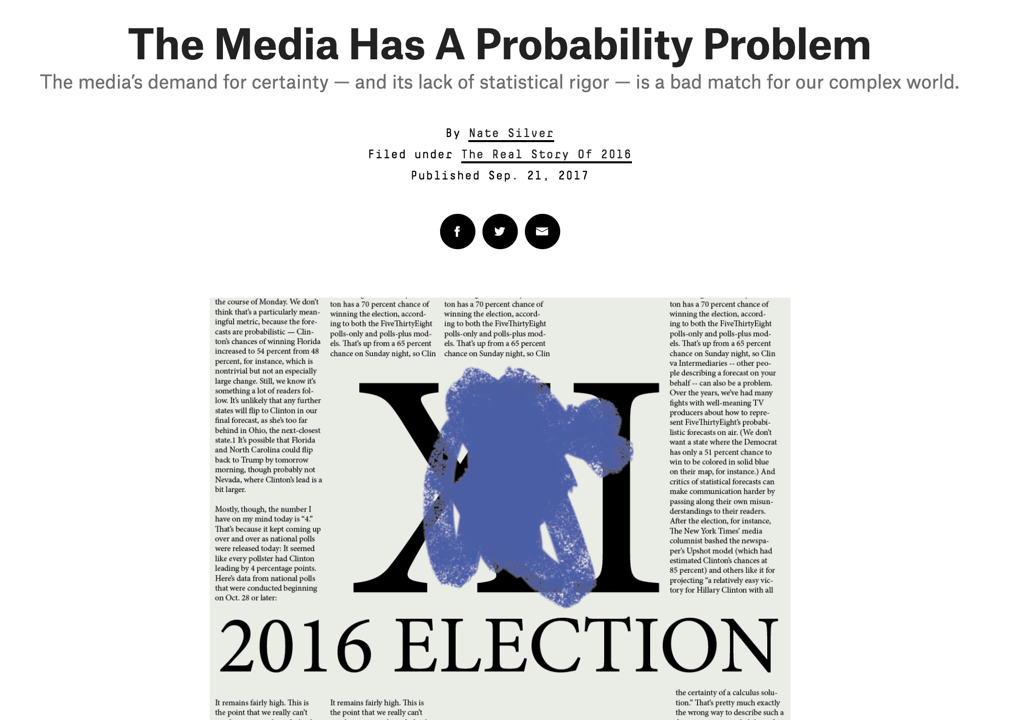
\includegraphics[width=8cm]{/Users/florianhollenbach/Documents/GitHub/Polisci209_2018/slides/week9/media_prob.png}
\end{center}
\end{frame}

\begin{frame}[label={sec:orgfb5dc11}]{Why probability?}
\begin{itemize}
\item What are the chances it rains tomorrow?
\end{itemize}

\pause

\begin{itemize}
\item What are the chances you win the lottery?
\end{itemize}

\pause

\begin{itemize}
\item What is the probabilty of getting an A in pols 209?
\end{itemize}
\end{frame}

\begin{frame}[label={sec:org79a4c57}]{Why probability?}
\begin{itemize}
\item We use probability to express and calculate uncertainty

\item \emph{Preview}: later we will use probability to make statements about the uncertainty in our data analysis
\end{itemize}
\end{frame}

\begin{frame}[label={sec:orgd6e35f2}]{Two fundamental concepts of probability}
\begin{itemize}
\item Frequentist: long-run frequency of events
\begin{itemize}
\item \alert{ratio between the number of times the event occurs and the number of trials}
\item example: coin flips
\end{itemize}
\end{itemize}

\pause

\begin{itemize}
\item Bayesian: belief about the likelihood of event occurrence
\begin{itemize}
\item evidence based belief
\item often more sensible philosophy in political world
\end{itemize}
\end{itemize}
\end{frame}

\begin{frame}[label={sec:org1fbc331}]{Important Terms}
\begin{enumerate}
\item \alert{Experiment}: an action or a set of actions that produce stochastic events of interest
\end{enumerate}

\pause

\begin{enumerate}
\item \alert{sample space}: a set of all possible outcomes of the experiment, typically denoted by \(\Omega\)
\end{enumerate}

\pause

\begin{enumerate}
\item \alert{event}: a subset of the sample space
\end{enumerate}

(Imai - QSS)
\end{frame}

\begin{frame}[label={sec:org202bf1d}]{Example}
What is the experiment, sample space, and one event for coin flips or pulling a single card out of a deck of 52?
\end{frame}

\begin{frame}[label={sec:orgee3abfc}]{Defining Probability}
Probability of event A = P(A) = \(\frac{\text{number of elements in A}}{\text{number of elements in sample space}}\)

\pause

Probability of Head = P(H) = \(\frac{1}{2}\)
\end{frame}


\begin{frame}[label={sec:org59c281a}]{Example}
What is the probability of 3 head in 3 flips?

Sample space?

\pause

\(\Omega\) = \{HHH,HHT,HTH,THH, HTT, THT, TTH, TTT\}

\pause

What is the event space we are interested in?

\pause

\{HHH\}
\end{frame}

\begin{frame}[label={sec:org5e0b658}]{Example}
What is the probability of 3 head in 3 flips?


\pause

P(HHH) = \(\frac{1}{8}\)
\end{frame}


\begin{frame}[label={sec:org24e8236}]{Example}
What is the probability of 2 head in 3 flips?

\(\Omega\) = \{HHH,HHT,HTH,THH, HTT, THT, TTH, TTT\}

What is the event space we are interested in?

\pause

\{HHT, HTH, THH\}

\pause

P(2 H) = \(\frac{3}{8}\)
\end{frame}

\begin{frame}[label={sec:org22dc5d5}]{Axioms (rules) of Probability}
\begin{itemize}
\item the probability of \alert{any} event A is at least 0
\begin{itemize}
\item P(A) \(\geq\) 0
\end{itemize}
\end{itemize}

\pause

\begin{itemize}
\item The total sum of all possible outcomes in the sample space must be 1
\begin{itemize}
\item P(\(\Omega\)) = 1
\end{itemize}
\end{itemize}

\pause

\begin{itemize}
\item If A and B are mutually exclusive (\alert{meaning only one or the other can happen}), then P(A or B) = P(A) + P(B)
\end{itemize}
\end{frame}


\begin{frame}[label={sec:org7d5660f}]{Axioms (rules) of Probability}
A\(^{\text{c}}\) - complement to A, i.e. part of sample space not in A

Sometimes it is easier to calculate the probability of an event by using its complement
\end{frame}



\begin{frame}[label={sec:org6db4849}]{Using the complement:}
What is the probability of having at least one Tail on three coin flips?

\(\Omega\) = \{HHH,HHT,HTH,THH, HTT, THT, TTH, TTT\}

\pause

P(at least one T) = \(\frac{7}{8}\)

P(at least one T) = 1 - P(HHH) = 1 - \(\frac{1}{8}\)
\end{frame}



\begin{frame}[label={sec:orgc37cb4c}]{Example of simple probability}
What is the probability of getting a Queen as the first card from a full deck?

\(\Omega\) = \{?\}

Event space = \{?\}


\pause

p(Queen) = \(\frac{4}{52} = \frac{1}{13}\)
\end{frame}




\begin{frame}[label={sec:org9d8af82}]{How to quickly count the sample space when order matters: permutations}
\begin{itemize}
\item Often we do not want to or can't write out all possible combinations by hand

\item How many possibilities are there to arrange letters A,B,C?
\end{itemize}

\pause

Three outcomes: A, B, C \& three draws

\pause
First draw: A,B, or C

Second draw: two possibilities

Third draw: one left

3 x 2 x 1 possibilities
\end{frame}

\begin{frame}[label={sec:org66cd648}]{How to quickly count the sample space when order matters: permutations}
Permutations count many ways we can \alert{order} k objects out of a set of n unique objects

\(_{n}P_{k} = n \times (n-1) \times (n-2) \times ... \times (n-k + 1) = \frac{n!}{(n-k)!}\)

What does n! stand for?

\pause

n! = n-factorial = \(n \times (n-1) \times (n-2) \times ... \times (n-n+1)\)

\(3! = 3 \times 2 \times 1\)

\alert{Note: 0! = 1}
\end{frame}


\begin{frame}[label={sec:orgf5e8b40}]{Permutation Example:}
How many ways can we arrange four cards out of a the 13 spades in our card deck?

first draw: ?
\pause

13 \texttimes{} 12 \texttimes{} 11 \texttimes{} 10

\pause

\(\frac{13!}{(13-4)!} = \frac{13!}{9!} = \frac{13 \times 12 \times 11 \times ... \times 2 \times 1}{9 \times 8 \times ... \times 2 \times 1} = 13 \times 12 \times 11 \times 10 = 17,160\)
\end{frame}

\begin{frame}[label={sec:org31aa2c0}]{Birthday Problem}
Impress your family over Thanksgiving!

\pause

What is the probability that at least two people in this room have the same birthday?

How could we figure that out?
\end{frame}

\begin{frame}[label={sec:orga1aacc3}]{Birthday Problem}
Can the law of total probabilities and complement help us?

\pause

Yes, P(at least two share bday) = 1 - P(nobody shares bday)
\end{frame}

\begin{frame}[label={sec:org8758f00}]{Birthday Problem}
P(nobody shares bday)?

What is the event space?

\pause

Event space:  everyone has a unique birthday. How many different possibilities?

\pause

How many possibilities for birthdays in a year?

\pause

365

\pause

How many unique arrangements would we need for nobody to share the birthday?

\emph{number of people in room - k}
\end{frame}

\begin{frame}[label={sec:org70331a2}]{Birthday Problem}
\begin{enumerate}
\item \(_{365}P_{k} = \frac{365!}{(365-k)!}\) possibilities to arrange k unique birthdays over 365 days

\item What is the sample space? \alert{All the different possibilities for k birthdays (even non-unique).}
\end{enumerate}

\pause
\(365^{k}\)
\end{frame}

\begin{frame}[label={sec:org51f3a5f}]{Birthday Problem}
P(at least two share bday) = 1 - P(nobody shares bday) = 1 - \(\frac{365!}{(365-k)! \times 365^{k}}\)

\pause

P(at least two share bday):

k = 10; 0.116,

k = 23; 0.504,

and k = 68; 0.999.
\end{frame}


\begin{frame}[label={sec:orgb715318}]{Combinations}
Combinations are similar to permutations, except that the ordering doesn't matter

So with respect to combinations of 3 out of 26 letters, ABC, BAC, CAB, etc are the same

\pause

There are \alert{always} fewer combinations than permutations
\end{frame}

\begin{frame}[label={sec:orga0f44fe}]{Combinations vs. Permutations}
Draw 2 out of letters ABC

Permutations:
\pause

AB, AC, BA, BC, CA, CB =  \(\frac{3!}{1!}\)

Combinations:

\pause

AB, AC, BC
\end{frame}

\begin{frame}[label={sec:orgf3563c3}]{How to Calculate Combinations}
Calculate permutations and then account for the fact that we overcounted due to ordering

Get rid of counts of different arrangements of same combination: divide by k!

\(_{n}C_{k} = {n \choose k} = \frac{_{n}P_{k}}{k!} = \frac{n!}{k!(n-k)!}\)


\pause
Why divide by k! ?

\pause
for two sampled elements, we have 2!(= 2×1 = 2): A, B = AB, BA
\end{frame}


\begin{frame}[label={sec:orgb4f8e4f}]{Lottery}
What is the probability of winning (simplified) Mega Millions?

Pick five numbers between 1 and 70

Probability of getting 5 correct?
\end{frame}


\begin{frame}[label={sec:orgc32eab6}]{Lottery}
Probability of getting 5 correct?

What is the size of the event space?

\pause

1 ticket
\end{frame}


\begin{frame}[label={sec:orgcffcb82}]{Lottery}
Pick five numbers between 1 and 70

Sample space?

\pause

\({70 \choose 5} = \frac{70!}{5! \times (70-5)!} =  \frac{70!}{5! \times 65!}\)


\pause

12,103,014
\end{frame}

\begin{frame}[fragile,label={sec:orgccd6276}]{Lottery}
 \({n \choose k}\) in \emph{R}

choose(n,k)

\begin{verbatim}
choose(70,5)
\end{verbatim}

\begin{verbatim}
[1] 12103014
\end{verbatim}
\end{frame}



\begin{frame}[label={sec:org33373e5}]{Samping \emph{with} and \emph{without} Replacement}
Two ways to sample (draw) data:

\begin{itemize}
\item with replacement: put draw back in box

\item without replacement: keep draw, ticket can \alert{not} be drawn again
\end{itemize}

\pause
If we are sampling for a survey, what technique do we use?
\end{frame}


\begin{frame}[label={sec:orgf6ffbaf}]{Simulating the birthday problem in \emph{R}}
\begin{itemize}
\item Instead of calculating probabilities, we can often simulate them in \emph{R}

\item Use \emph{R} to draw k birthdays and see whether any duplicates exist
\end{itemize}

\pause

\begin{itemize}
\item We repeat the experiment over and over (\textasciitilde{} 1000 times). The share of experiments in which we found duplicates, will represent P(at least one shared bday)
\end{itemize}
\end{frame}

\begin{frame}[fragile,label={sec:org46d5766}]{Simulating the birthday problem in \emph{R}}
 \begin{verbatim}
k <- 23 # number of people
sims <- 1000 # number of simulations
event <- 0 # counter
for (i in 1:sims) {
    days <- sample(1:365, k, replace = TRUE)
    days.unique <- unique(days) # unique birthdays
    if (length(days.unique) < k) {
        event <- event + 1 } }
event / sims
\end{verbatim}

\begin{verbatim}

[1] 0.499
\end{verbatim}
\end{frame}



\begin{frame}[fragile,label={sec:org7c40f45}]{Simulating the birthday problem in \emph{R}}
 The larger the number of simulation iterations, the better the accuracy
\begin{verbatim}
sims <- 10000 # number of simulations
event <- 0 # counter
for (i in 1:sims) {
    days <- sample(1:365, k, replace = TRUE)
    days.unique <- unique(days) # unique birthdays
    if (length(days.unique) < k) {
        event <- event + 1  }}
event / sims
\end{verbatim}

\begin{verbatim}

[1] 0.5181
\end{verbatim}
\end{frame}
\end{document}